\documentclass[11pt]{beamer}
\usepackage{booktabs} 
\usepackage{graphicx}
\usepackage[utf8]{inputenc} 
\usepackage[russian]{babel} 
\usepackage{bm}
\usepackage{indentfirst}
\usepackage{amsfonts}
\usepackage{amsmath}
\usepackage{amsthm}
\usepackage{bbold}
\usepackage{moreverb}
\usepackage{dsfont}
\usepackage[]{algorithm2e}
\mode<presentation> {
	%\usetheme{Warsaw}
	\useinnertheme[shadow]{rounded}
	\usecolortheme{wolverine}
	%\usecolortheme{crane}
}

\DeclareMathOperator{\tr}{tr}
\DeclareMathOperator*{\argmin}{arg\,min}
\DeclareMathOperator*{\argmax}{arg\,max}
\DeclareMathOperator{\sign}{sign}
\DeclareUnicodeCharacter{2212}{-}

\newcommand*\oldmacro{}%
\let\oldmacro\insertshorttitle%
\renewcommand*\insertshorttitle{%
	\oldmacro\hfill%
	\insertframenumber\,/\,\inserttotalframenumber}
\newcommand{\RomanNumeralCaps}[1]
{\MakeUppercase{\romannumeral #1}}
\begin{document}
	\title[Neural Nets]{Neural Nets (NN), с элементами Deep Learning}
	\author{Хасанова Кристина, Гриненко Юрий}
	
	\institute[] 
	{
		гр. 22.M03-мм \\
		Санкт-Петербургский государственный университет \\
		Кафедра статистического моделирования 
	}
	
	\begin{frame}
		\titlepage 
	\end{frame}

	\begin{frame}{Постановка задачи}
		Пусть $X$ --- множество объектов, $Y$ --- множество ответов. Пусть есть обучающая выборка $X^n = (x_i, y_i)_{i=1}^{n},$ $x_i \in \mathbb{R}^p$. Обозначим $(x^1,\ldots,x^p)\in \mathbb{R}^p$ --- вектор признаков объекта $x\in X$. Рассмотрим следующую задачу построения предсказывающей модели:
		\begin{equation*}
			Q(a, X^n) = \frac{1}{n} \sum_{i=1}^{n} \mathcal{L}(a,x_i,y_i) \rightarrow \min_w,
		\end{equation*}
	
		\pause
	
		где предсказывающую функцию $a$ зададим следующим образом (рассмотрим особый класс функций):
		\begin{equation*}
			a(x, w) = \sigma( \langle w,x \rangle ) = \sigma\left(\sum_{j=1}^{p} w_j x^j - w_0 \right),
		\end{equation*}
		где $w_k \in \mathbb{R}$, $k=0,\ldots,p$ --- параметры; 
		$\sigma: \mathbb{R} \rightarrow  \mathbb{R} $ --- функция активации;
		$\mathcal{L}(a,x_i,y_i)$ --- функция потерь, $i=1,\ldots,n$.
	\end{frame}

	\begin{frame}{Функции потерь в задачах классификации}
		\begin{figure}[hhh!]
			\begin{center}
				\includegraphics[width=10cm]{loss}
			\end{center}
			\vspace{-5mm}
		\end{figure}
	\end{frame}

	\begin{frame}{Основные задачи}
		
		\begin{equation*}
			a(x, w) = \sigma( \langle w,x \rangle ) = \sigma\left(\sum_{j=1}^{p} w_j x^j - w_0 \right),
		\end{equation*}
	
		Задача классификации. Пусть $Y=\{+1,-1\}$. Если $\sigma (z)=\sign(z)$, то $a(x,w)$ --- линейный классификатор, и задача выглядит следующим образом: 
		
		\begin{equation*}
			Q(w, X^{n})=\sum_{j=1}^{n} \mathcal{L} \left( a(x_j ,w), y_j \right) = \sum_{j=1}^{n} [y_j \langle w,x_j \rangle  < 0] \rightarrow \min_{w}.
		\end{equation*}
		
		Задача регрессии. Пусть $Y=\mathbb{R}$. Если взять $\sigma(z)=z$, то получим многомерную линейную регрессию:
		\begin{equation*}
			Q(w, X^{n})=\sum_{j=1}^{n} \mathcal{L} \left( a( x_j,w ), y_j \right)=\sum_{j=1}^{n}\left( \langle w,x_j \rangle  -y_j \right)^2 \rightarrow \min_{w}.
		\end{equation*}
	\end{frame}

	\begin{frame}{Нейрон}
		Рассмотренный класс функций удобно представить схематически. Такой класс функций является простейшей математической моделью нервной клетки --- нейрона.
		
		Если $\sigma = [z\geq0]$, то $\sigma\left(\sum_{j=1}^{p} w_j x^j - w_0 \right)$-- нейрон МакКаллока-Питтса. 
		
	\begin{figure}[hhh!]
		\begin{center}
			\includegraphics[width=10cm]{neur1}
		\end{center}
		\vspace{-5mm}
	\end{figure}

	\end{frame}

	\begin{frame}{Функции активации}
		В качестве функций активации чаще всего используются следующие функции:
		\begin{itemize}
			\item Сигмоидная функция: $\sigma(z) = \frac{1}{1+e^{-a\,z}}$, $a \in \mathbb{R}$;
			\item Softmax: $SM_i(z)  = \frac{e^{z_i}}{\sum_{k=1}^{K}e^{z_k}}$;
			\item Гиперболический тангенс: $\sigma(z) = \frac{e^{a\,z} - e^{-a\,z}}{e^{a\,z} + e^{-a\,z}}$, $a \in \mathbb{R}$;
			\item Выпрямитель: $ReLU(p) = \max (0,p)$;
		\end{itemize}
			

		\begin{figure}[hhh!]
			\begin{center}
				\includegraphics[width=10cm]{activation}
			\end{center}
			\vspace{-5mm}
		\end{figure}
		
	\end{frame}

	\begin{frame}{Операция 'НЕ'}
		Логическая операция 'НЕ' может быть представлена в виде $\lnot x^1 = [-x^1+\frac{1}{2}>0]$. Далее представлен нейрон, реализующий эту операцию.
		
		\begin{figure}[H]
			\begin{center}
					\includegraphics[width=250pt, height=70pt]{boolean1}
					\caption{Представление логической операции 'НЕ' в виде нейрона.}
					\label{bool1}
			\end{center}
		\end{figure}
	\end{frame}

	\begin{frame}{Операции 'ИЛИ', 'И'}
		Логические операции 'ИЛИ', 'И' могут быть представлены в таком виде: $x^1 \lor x^2 = [x^1+x^2 -\frac{1}{2}>0]$ и $x^1 \wedge x^2 = [x^1+x^2 -\frac{3}{2}>0]$. Далее представлены нейроны, реализующие эти булевы функции.
		
		\begin{figure}[H]
			\begin{center}
					\includegraphics[width=300pt, height=100pt]{boolean2}
					\caption{Представление логических операций 'ИЛИ' и 'И' в виде нейронов.}
					\label{bool2}
			\end{center}
		\end{figure}
	\end{frame}

	\begin{frame}{'Исключающее ИЛИ'}
		Такая операция не может быть реализована одним нейроном с двумя входами $x^1$ и $x^2$. Возможны два варианта решения такой задачи. 
		
		Первый вариант --- пополнить пространство признаков, добавить нелинейное преобразование исходных признаков. Например, если добавить произведение исходных признаков, тогда нейрон будет строить уже не линейную, а полиномиальную разделяющую поверхность. Таким образом, мы перейдем к спрямляющему пространству признаков. Функцию "исключающего ИЛИ"$~$ можно представить в виде $x^1 \oplus x^2 = [x^1+x^2 -2x^1x^2-\frac{1}{2}>0]$, схема нейрона представлена на рисунке.
	\end{frame}

	\begin{frame}{'Исключающее ИЛИ'}
		\begin{figure}[H]
			\begin{center}
					\includegraphics[width=300pt, height=90pt]{boolean3}
					\caption{Представление логической операции 'исключающее ИЛИ' $~$ в виде одного нейрона.}
					\label{bool3}
			\end{center}
		\end{figure}
	\end{frame}

	\begin{frame}{'Исключающее ИЛИ'}
		Второй вариант --- построить композицию из нескольких нейронов. Например, 'исключающее ИЛИ'$~$ можно представить в таком виде: $x^1 \oplus x^2 = [\lnot((x^1\lor x^2) - (x^1 \wedge x^2))>0]$. Получаем суперпозицию нейронов --- нейронную сеть.
		
		\begin{figure}[H]
			\begin{center}
					\includegraphics[width=300pt, height=100pt]{boolean4}
					\caption{Представление логической операции 'исключающее ИЛИ' $~$ в виде суперпозиции нейронов.}
					\label{bool4}
			\end{center}
		\end{figure}
	\end{frame}

	\begin{frame}{Насколько богатый класс функций может быть реализован нейроном}
		\begin{theorem}[Цыбенко, 1989]
			Пусть $\sigma(x)$ --- ограниченная и монотонно возрастающая непрерывная функция; $C(I_{p_0})$ --- множество непрерывных функций на $[0,1]^{p_0}$.
			
			Тогда $\forall f \in C(I_{p_0})$ и $\forall \varepsilon > 0$  $\exists ~p_1 \in \mathbb{Z}$ и  $\alpha_i$, $b_i$, $w_{ij} \in \mathbb{R}$, $i=1,\ldots,p_1$, $j=1,\ldots, p_0$, такие что для любого $x=(x^1, \ldots, x^{p_0}) \in I_{p_0}$ выполняется
			\begin{equation*}
				| F(x^1, \ldots, x^{p_0}) - f(x^1, \ldots, x^{p_0})| < \varepsilon,
			\end{equation*}
			где  \begin{equation*}
				F(x^1, \ldots, x^{p_0})=\sum_{i=1}^{p_1} \alpha_i \, \sigma \left(\sum_{j=1}^{p_0} w_{ij} x^j -w_{0i}   \right).
			\end{equation*}
		\end{theorem}	
	\end{frame}

	\begin{frame}{Следствия}
			Верно следующее:
		\begin{enumerate} 
			\item Двухслойная сеть в $\{0,1\}^n$ позволяет реализовать любую булеву функцию (ДНФ). 
			\item Двухслойная сеть в $\mathbb{R}^n$ позволяет реализовать любой выпуклый многогранник. 
			\item Трехслойная сеть в $\mathbb{R}^n$ позволяет отделить любую многогранную область, не обязательно выпуклую и не обязательно связную. 
			\item С помощью линейных операций и одной нелинейной функции активации можно приблизить любую непрерывную функцию с любой точностью (теорема Горбаня, 1998). 
		\end{enumerate}
	\end{frame}

	\begin{frame}{Алгоритм обратного распространения ошибки BackProp}
		\begin{figure}[H]
			\begin{center}
					\includegraphics[width=270pt, height=140pt]{neuralnetwork}
					\caption{Двухслойная нейронная сеть}
					\label{neuralnetwork}
			\end{center}
		\end{figure}
	В случае двухслойной сети: $a^m(x_i)$, $m=1,\ldots,M$ на объекте $x_i$:
	\begin{equation*}
		a^m(x_i) = \sigma_m \left(\sum_{h=0}^{H} w_{hm}  u^h(x_i)  \right), ~~~~~~
		u^h(x_i) = \sigma_h \left(\sum_{j=0}^{p} w_{jh} x_{i}^j   \right).
	\end{equation*}
	\end{frame}
	
	\begin{frame}{Проблема оптимизации}
		В случае двухслойной нейронной сети получим $(p+1)H+(H+1)M$ весовых коэффициентов. Для решения поставленной задачи используются градиентные методы, в частности, стохастический градиентный спуск, однако при таком большом количестве параметров посчитать градиент довольно трудоемко. Для решения этой проблемы возник метод обратного распространения ошибки, который с некоторыми затратами памяти эффективно вычисляет градиент.
	\end{frame}

	\begin{frame}
		Для начала поставим промежуточную задачу эффективного вычисления частных производных $\frac{\partial \mathcal{L}_i(w)}{\partial a^m}$ и $\frac{\partial \mathcal{L}_i(w)}{\partial u^h}$. Идея состоит в том, что при первом вычислении сети мы будем сохранять некоторые величины, которые впоследствии помогут быстро посчитать градиент.
		
		В случае двухслойной сети: $a^m(x_i)$, $m=1,\ldots,M$ на объекте $x_i$:
		\begin{equation*}
			a^m(x_i) = \sigma_m \left(\sum_{h=0}^{H} w_{hm}  u^h(x_i)  \right), ~~~~~~
			u^h(x_i) = \sigma_h \left(\sum_{j=0}^{p} w_{jh} x_{i}^j   \right).
		\end{equation*}
		Пусть для конкретности
		\begin{equation*}
			\mathcal{L}_i(w) = \frac{1}{2} \sum_{m=1}^{M}(a^m(x_i) - y^m_i)^2,
		\end{equation*}
		для других функций потерь рассуждения можно провести по аналогии.
	\end{frame}

	\begin{frame}{Ошибки на выходном и промежуточном слоях}
		Выпишем выражения для частных производных. Для краткости записи будем обозначать $\sigma'_m = \sigma'_m (\sum\limits_{h=0}^H w_{hm} u^h(x_i))$ и аналогично для других производных в соответствующих точках.
		\begin{equation*}
			\frac{\partial \mathcal{L}_i(w)}{\partial a^m} = a^m(x_i) - y_i^m = \varepsilon^m_i ~~\text{ --- ошибка на выходном слое,}
		\end{equation*}
		
		\begin{equation*}
			\frac{\partial \mathcal{L}_i(w)}{\partial u^h} = \sum \limits_{m=1}^M (a^m(x_i) - y_i^m) \sigma_m' w_{hm} = \sum \limits_{m=1}^M \varepsilon^m_i \sigma_m' w_{hm} = \varepsilon^h_i.
		\end{equation*}
		По аналогии назовем это также ошибкой на нейроне промежуточного слоя.
	\end{frame}

	\begin{frame}{Вычисление $\varepsilon$}
		Теперь заметим, что $\varepsilon_i^h$ вычисляется по $\varepsilon_i^m$, если запустить сеть в обратном порядке, справа налево:
		
		\begin{center}
			\centering
			\includegraphics[width=220pt, height=100pt]{backprop}
		\end{center}
	\end{frame}

	\begin{frame}{Формулы для компонент вектора градиента}
		Итак, имеем формулы для компонент вектора градиента:
		\begin{equation*}
			\frac{\partial \mathcal{L}_i(w)}{\partial w_{hm}} = \frac{\partial \mathcal{L}_i(w)}{\partial a^m} \frac{\partial a^m}{\partial w_{hm}} =   \varepsilon^m_i \sigma_m' u^h(x_i), ~~~~~ h=0,\ldots,H, ~~ m=1,\ldots,M,
		\end{equation*}
		
		\begin{equation*}
			\frac{\partial \mathcal{L}_i(w)}{\partial w_{jh}} = \frac{\partial \mathcal{L}_i(w)}{\partial u^h} \frac{\partial u^h}{\partial w_{jh}} =   \varepsilon^h_i \sigma_h' f_j(x_i), ~~~~~ j=0,\ldots,p, ~~ h=1,\ldots,H.
		\end{equation*}
		
		Будем сохранять промежуточные величины $\varepsilon_i^m$ и $\varepsilon_i^h$, чтобы эффективно вычислить компоненты вектора градиента. Полученный алгоритм --- это метод стохастического градиентного спуска с быстрым вычислением градиента. \\
	\end{frame}

	\begin{frame}{Обучение двухслойной нейронной сети методом обратного распространения ошибки (back-propagation)}
		\fontsize{9.5}{7.2}\selectfont
		\begin{algorithm}[H]
			\SetAlgoLined
			\KwIn{$\mathbb{X}^n=\{x_i, y_i\}_{i=1}^n$ --- обучающая выборка, $x_i \in \mathbb{R}^p$, $y_i \in \mathbb{R}^M$, $H$ --- число нейронов на скрытом слое, $\eta$ --- темп обучения, параметр $\lambda$}
			\KwOut{$w_{jh}, w_{hm}$ --- веса}
			
			Инициализация весов $w_{jh},~ w_{hm}$\;
			\Repeat{$Q$ не сойдется}{
				Выбираем $x_i$ из $\mathbb{X}^n$\;
				Прямой ход: 
				\newline
				$u^h:=\sigma_h(\sum\limits_{j=0}^n w_{jh}x_i^j), ~~~ h=1,\ldots,H$;
				\newline
				$a^m:=\sigma_m(\sum\limits_{h=0}^H w_{hm}u_i^h),~~ \varepsilon_i^m:=a_i^m-y_i^m, ~~~ m=1,\ldots,M$; 
				\newline
				$\mathcal{L}_i:=\sum\limits_{m=1}^M (\varepsilon_i^m)^2$ \;
				Обратный ход: $\varepsilon_i^h:= \sum\limits_{m=1}^M \varepsilon_i^m\sigma_m' w_{hm}, ~~~ h=1,\ldots,H$\;
				Градиентный шаг: 
				$w_{hm}:=w_{hm}-\eta \varepsilon_i^m \sigma_m' u^h(x_i), ~~~~~~ h=0,\ldots,H, ~ m=1,\ldots,M$;
				$w_{jh}:=w_{jh}-\eta \varepsilon_i^h \sigma_h' f^j(x_i), ~~~~~~ j=0,\ldots,p, ~ h=1,\ldots,H$ \;
				$Q:=(1-\lambda)Q+\lambda\mathcal{L}_i$;		
			}
		\end{algorithm}
	\end{frame}

	\begin{frame}{Достоинства и недостатки}
		\textbf{Достоинства} метода обратного распространения ошибок:
		\begin{itemize}
			\item эффективность: быстрое вычисление градиента. В случае двухслойной сети прямой ход, обратный ход и вычисление градиента требуют порядка $O(Hp+HM)$ операций;
			\item метод легко обобщается на любые функции потерь, функции активации, произвольное количество слоев и произвольную размерность входов и выходов;
			\item возможно динамическое (потоковое) обучение;
			\item на сверхбольших выборках не обязательно брать все $x_i$.
		\end{itemize}
		
		\textbf{Недостатки} (есть все те же, что и у метода стохастического градиента):
		\begin{itemize}
			\item метод не всегда сходится;
			\item возможна медленная сходимость;
			\item застревание в локальных минимумах;
			\item проблема переобучения.
		\end{itemize}
	\end{frame}

	\begin{frame}{Инициализация весов}
		\begin{itemize}
			\item Часто веса инициализируются случайно, небольшими по модулю значениями. Например, в качестве начального приближения берутся случайные значения из отрезка $[-\frac{1}{2k}, \frac{1}{2k}]$, где $k$ --- число нейронов в том слое, из которого выходит связь.
			\item Существует вариант инициализации весов в зависимости от корреляции признака и столбца ответов:
			\begin{equation*}
				w_{jh}=\frac{\langle x^j, y\rangle}{\langle x^j, x^j\rangle} + \varepsilon_{jh}.
			\end{equation*}
			
			\item Начальное приближение также можно сформировать по-другому. Идея заключается в том, чтобы сначала настроить нейроны первого слоя отдельно, как H однослойных нейронных сетей.
		\end{itemize}
	\end{frame}

	\begin{frame}{Выбор градиентного метода}
		\begin{itemize}
			\item \textbf{Метод стохастического градиента с адаптивный шагом.}:
			\begin{equation*}
				Q(w - \eta \frac{\delta Q}{\delta w}) \rightarrow \min_\eta.
			\end{equation*}

			\item Adagrad:
			\begin{equation*}
				G_{k+1} = G_k + (\nabla f(x_k))^2 
			\end{equation*}
			
			\begin{equation*}
				x_{k+1} = x_k - \frac{\alpha}{\sqrt(G_{k+1} + \epsilon)} \nabla f(x_k)
			\end{equation*}
			\item RMSProp
				\begin{equation*}
					G_{k+1} = \gamma G_k + (1 - \gamma G_k)(\nabla f(x_k))^2 x_{k+1}
				\end{equation*}
		
				\begin{equation*}
					x_{k+1} = x_k - \frac{\alpha}{\sqrt(G_{k+1} + \epsilon)} \nabla f(x_k)
				\end{equation*}
		\end{itemize}
	\end{frame}
	
	\begin{frame}{Выбор градиентного метода}
		\begin{itemize}

			\item Adam: 
			\begin{equation*}
				x_{k+1} = x_k - \frac{\alpha}{\sqrt(G_{k+1} + \epsilon)} v_{k+1}
			\end{equation*}
			
			\begin{equation*}
				v_{k+1} = \beta_1 v_k - (1 - \beta_1 v_k)  \nabla f(x_k)
		    \end{equation*}
			
			\begin{equation*}
				G_{k+1} = \beta_2 G_k + (1 - \beta_2 G_k)(\nabla f(x_k))^2 x_{k+1}
			\end{equation*}
		
	   \end{itemize}
	
		\begin{center}
			\begin{minipage}{0.51\linewidth}
				\centering
				\includegraphics[width=220pt, height=100pt]{optimizers}
			\end{minipage}
		\end{center}

	\end{frame}

	\begin{frame}{Выбор числа слоёв в случае классификации} 
		Если знаем, что классы линейно разделимы, то нам достаточно ограничиться одним слоем. Если граница между классами нелинейная и извилистая, то в большинстве случаев достаточно взять двухслойную сеть. Трёхслойными сетями имеет смысл пользоваться для представления сложных многосвязных областей. Теоретически, можно взять нейронную сеть с большим количеством слоев, однако тогда хуже сходятся градиентные методы, и тем труднее нам будет её обучить.
	\end{frame}

	\begin{frame}{Выбор числа нейронов в скрытом слое (выбор H)}
		\begin{enumerate}
			\item Визуальный способ. Если граница классов (или кривая регрессии) слишком сглажена --- количество нейронов в слое нужно увеличить, а если есть резкие колебания, то, наоборот, уменьшить. Этот способ подходит для задач с небольшим числом признаков.
			\item По внешнему критерию. Можно смотреть на среднюю ошибку на тестовой выборке или использовать cross-validation. Недостаток этого способа --- высокая трудоёмкость. Приходится много раз заново строить сеть при различных значениях параметра $H$, а в случае скользящего контроля --- ещё и при различных разбиениях выборки на обучающую и контрольную части.
		\end{enumerate}
	\end{frame}

	\begin{frame}{Динамическое наращивание сети}
			\begin{enumerate}
			\item Обучение сети при заведомо недостаточном числе нейронов $H \ll n$, пока ошибка не перестаёт убывать;
			\item Добавление нового нейрона и его инициализация путем обучения 
			\begin{itemize}
				\item либо по случайной подвыборке $X^{'} \subseteq X^n$;
				\item либо по объектам с наибольшими значениями потерь;
				\item либо по случайному подмножеству входов;
				\item либо из различных случайных начальных приближений.
			\end{itemize}
			\item Снова итерации BackProp;
		\end{enumerate}
	\end{frame}

	\begin{frame}{Выбор числа эпох обучения}
		\textbf{Выбор числа эпох обучения.} Алгоритм работы нейронной сети является итеративным, его шаги называют эпохами или циклами. Эпоха - одна итерация в процессе обучения. Обычно, чем больше количество эпох, тем меньше лосс на обучающей выборке.
		Ниже можно увидеть сравнение динамики лосса для обучающей и валидационной выборки.
	
		\begin{center}
			\begin{minipage}{0.51\linewidth}
				\centering
				\includegraphics[width=220pt, height=100pt]{losses}
			\end{minipage}
		\end{center}

	\end{frame}

	\begin{frame}{Разновидности нейронных сетей I}
		\begin{itemize}
			\item Сеть прямого распространения (Feed Forward).
			\begin{center}
				\begin{minipage}{0.51\linewidth}
					\centering
					\includegraphics[width=220pt, height=100pt]{ff}
				\end{minipage}
			\end{center}
		
			\item Сеть радиальных базисных функций (RBFN).
						
		\end{itemize}
	\end{frame}
			
	\begin{frame}{Разновидности нейронных сетей II}
		\begin{itemize}
			\item Рекуррентные нейронные сети (RNN).
			\begin{center}
				\begin{minipage}{0.51\linewidth}
					\centering
					\includegraphics[width=220pt, height=100pt]{rnn}
				\end{minipage}
			\end{center}

			\item Долгая краткосрочная память (LSTM).
			\begin{center}
				\begin{minipage}{0.51\linewidth}
					\centering
					\includegraphics[width=220pt, height=100pt]{lstm}
				\end{minipage}
			\end{center}
			
		\end{itemize}
	\end{frame}
	
	\begin{frame}{Разновидности нейронных сетей III}
		\begin{itemize}
			\item Деконволюционные сети (DNN).
			\item Сверточные нейронные сети (CNN).
			\begin{center}
				\begin{minipage}{0.51\linewidth}
					\centering
					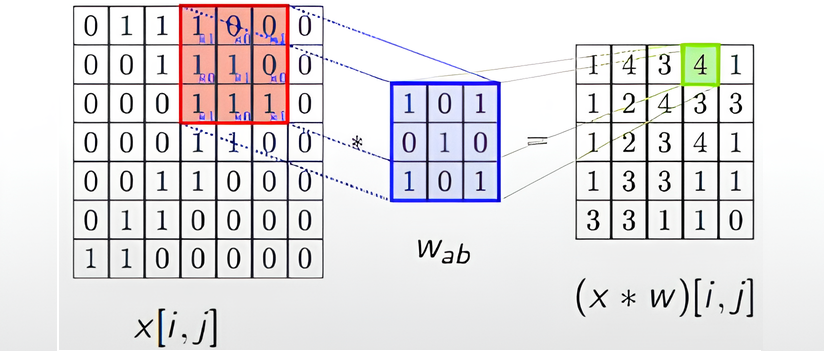
\includegraphics[width=220pt, height=100pt]{cnn}
			    \end{minipage}
		    \end{center}
			
	    \end{itemize}
		
	\end{frame}

	\begin{frame}{Разновидности нейронных сетей IV}
		\begin{itemize}
			\item Автоэнкодер.
		    \begin{center}
				\begin{minipage}{0.51\linewidth}
					\centering
					\includegraphics[width=220pt, height=100pt]{autoencoder}
				\end{minipage}
			\end{center}
			
			\item Генеративно-состязательные сети (GAN).
			\begin{center}
				\begin{minipage}{0.51\linewidth}
					\centering
					\includegraphics[width=220pt, height=100pt]{gan}
				\end{minipage}
			\end{center}
		\end{itemize}
	\end{frame}
	
	
	\begin{frame}{Разновидности нейронных сетей V}
		\begin{itemize}			
			\item transformer.
			\begin{center}
				\begin{minipage}{0.51\linewidth}
					\centering
					\includegraphics[width=220pt, height=220pt]{transformer}
				\end{minipage}
			\end{center}
		\end{itemize}
		
	\end{frame}

	\begin{frame}{Глубокое обучение в парадигме методов машинного обучения}
		\begin{figure}[H]
			\begin{center}
				\includegraphics[width=0.9\linewidth]{deepl}
			\end{center}
			\caption{Отличие между машинным обучением и глубоким обучением}
		\end{figure}
	\end{frame}

  \begin{frame}{Рекуррентные нейронные сети (RNN)}
	Рассмотрим устройство рекуррентных нейронных сетей. 
	Пусть $\boldsymbol{x}_t$ — входной вектор в момент времени $t$,\\ $\boldsymbol{h}_t$ — вектор скрытого состояния в момент времени $t$,\\
	$\boldsymbol{y}_t$ — выходной вектор в момент времени $t$. Стоит заметить, что в некоторых приложениях
	$\boldsymbol{y}_t \equiv \boldsymbol{h}_t$. \\
	Разворачивание рекуррентной нейронной сети:
	$\boldsymbol{h}_t = \sigma_h(Ux_t + Wh_{t-1})$\\
	$\boldsymbol{y}_t = \sigma_y (Vh_t) $ 
	    \begin{figure}
	        \centering
	        \includegraphics[width=230pt, height=90pt]{RNN1.png}
	        \caption{Рекуррентная нейронная сеть}
	        \label{fig:my_label}
	    \end{figure}


	\end{frame}

	\begin{frame}{ Обучение рекуррентной сети RNN}
		Возникает задача минимизации следующего функционала:

		\begin{equation*}
		\sum_{t=0}^{T} \mathcal{L}_t (\mathbf{U}, \mathbf{V}, \mathbf{W}) \rightarrow \min_{\mathbf{U},\mathbf{ V}, \mathbf{W}},
		\end{equation*}
		где $\mathcal{L}_t (\mathbf{U}, \mathbf{V}, \mathbf{W}) = \mathcal{L} (y_t(\mathbf{U}, \mathbf{V}, \mathbf{W}))$ --- функция потерь от предсказания $\hat{y}_t$.

		Используется вариант обратного распространения ошибок --- Backpropagation Through Time (BPTT):
		\begin{equation*}
			\dfrac{\partial \mathcal{L}_t}{\partial \mathbf{W}} = \dfrac{\partial \mathcal{L}_t}{\partial y_t} \dfrac{\partial y_t}{\partial h_t} \sum_{k=0}^t \left( \prod_{i = k + 1}^t \dfrac{\partial h_i}{\partial h_{i-1}} \right) \dfrac{\partial h_k}{\partial \mathbf{W}}.
		\end{equation*}

		Проблема:
		Затухание/взрыв градиентов, если $\frac{\partial h_i}{\partial h_{i-1}}\nrightarrow 1$, нужно ограничить частную
		производную(ввести архитектуру, чтобы эта величина стремилась к 1)
	\end{frame}

 	\begin{frame}{LSTM (long short-term memory)}
 		Мотивация LSTM: сеть должна долго помнить контекст, какой именно —
		сеть должна выучить сама. Поэтому вводится $C_t$ — вектор состояния сети
		в момент $t$.
      	\begin{figure}
	        \centering
	        \includegraphics[scale=0.32]{lstm1.png}  
	    \end{figure}
 	\end{frame}
 
 	\begin{frame}{LSTM (long short-term memory)}
		 \begin{figure}
	        \centering
	        \includegraphics[scale=0.32]{lstm2.png}
	    \end{figure}


		Фильтр забывания (forget gate) с параметром $W_f$, $b_f$ решает,
		какие координаты вектора $C_{t−1}$ надо запомнить.

		$\odot$ -- операция покомпонентного перемножения векторов,\\$[h_{t-1},x_t]$ конкатенация векторов,\\
		$\sigma$ сигмоидная функция.
 	\end{frame}
 
 
 	\begin{frame}{LSTM (long short-term memory)}
      	\begin{figure}
	        	\centering
	        	\includegraphics[scale=0.32]{lstm3.png}
	    	\end{figure}
     	Фильтр входных данных (input gate) с параметром $W_i$, $b_i$ решает,
		какие координаты вектора состояния надо обновить.\\
		Модель нового состояния с параметрами $w_C$, $b_C$ формирует вектор $\widetilde{C}_t$ значений-координатов нового состояния.
 	\end{frame}
 
 	\begin{frame}{LSTM (long short-term memory)}
      	\begin{figure}
	        \centering
	        \includegraphics[scale=0.32]{lstm4.png}
	        
	    \end{figure}
    	Новое состояние $C_t$ формируется как смесь старого состояния $C_{t-1}$ с фильтром $f_t$ и вектора значений-кандидатов $\widetilde{C}_t$ c фильтром $i_t$.\\
    	Настраиваемых параметров нет.
 	\end{frame}

 	\begin{frame}{LSTM (long short-term memory)}
      	\begin{figure}
	       	 \centering
	        	\includegraphics[scale=0.32]{lstm5.png}
	        
	    \end{figure}
     	Фильтр входных данных с параметрами $W_o$, $b_o$ решает какие координаты вектора состояния $C_t$ надо выбрать.\\
    	Выходной сигнал $h_t$ формируется из вектора состояния $C_t$ с помощью нелинейного преобразования $th$ и фильтра $o_t$.
 	\end{frame}

\end{document} 